\subsection{Radiation and Scattering}

\subsubsection{Electric Dipole Radiation}\label{Electric Dipole Radiation}

As always, the first we should do is to sketch the system we want to study;

\begin{figure}[h]
	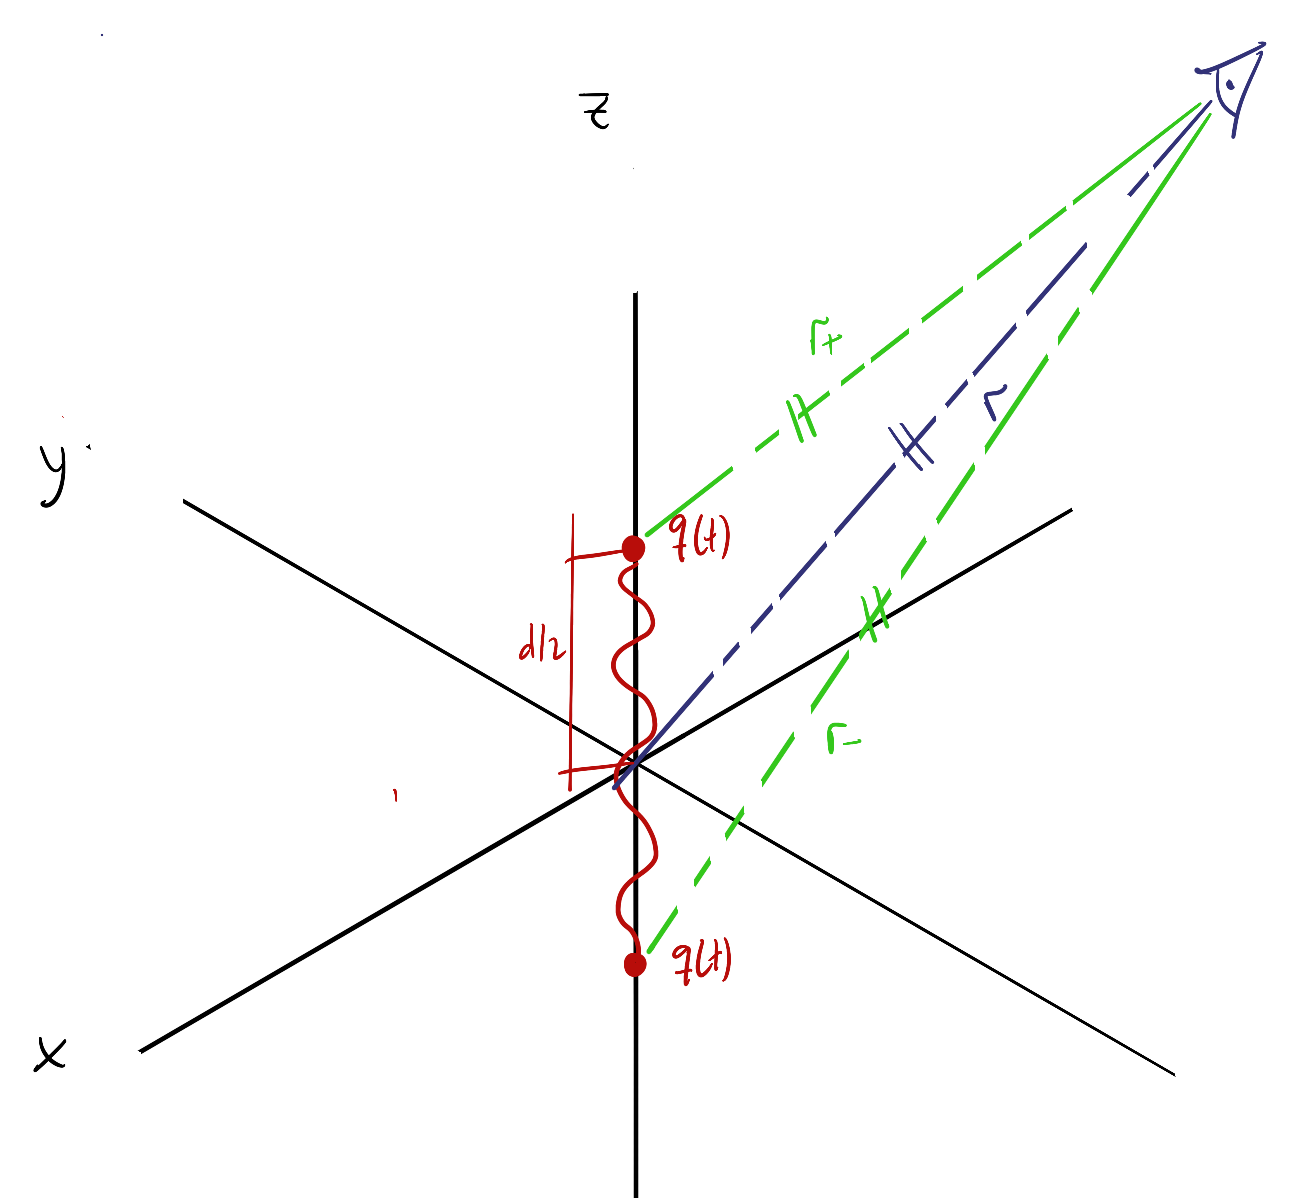
\includegraphics[width=8cm]{figures/Dipolerad.png}
	\centering
	\caption{Our time dependant dipole.}
\end{figure}

Where $q(t)= q_{0} \cos \omega t$. We can compute the potential as a superposition of both charges as:

\begin{equation}
	V(r) = \sum_{i=0}^{n} \frac{q_{i}}{4\pi \epsilon_{0}r_{i}}=\frac{q(t)}{4\pi \epsilon_{0}r_{1}} - \frac{q(t)}{4\pi \epsilon_{0}r_{2}}.
\end{equation}

As we can see in the sketch, there is a difference in the paths $r_{i}$. If we are \textit{Far Far away}\footnote{With Fiona and her parents.}, we can always approximate $r \gg \tfrac{d}{2}$, which will allow us to expand the norm of $\vec{r}_{i}$ as:

\begin{equation}
	|\vec{r}_{i}| = \sqrt{(\vec{r} \pm (0,0,\tfrac{d}{2}))^{2}} \approx \sqrt{r^{2} + \tfrac{d^{2}}{4} \pm d r \cos \theta}.
\end{equation}

But one has also to consider that the change of charge in $r$ position will have a different delay depending on the path they have to travel. In this case we have to take into account the retarded time as:

\begin{equation}
	t_{\pm}= t - \tfrac{r_{\pm}}{c}.
\end{equation}

So the potential gets more involved with the following appearance:

\begin{equation}\label{pottosimp}
	V(r)= \frac{q_{0}}{4\pi \epsilon_{0}}\left[\tfrac{\cos (\omega (t -\tfrac{r_{+}}{c}))}{\sqrt{r^{2}+\tfrac{d^{2}}{4}+d r \cos\theta}} - \tfrac{\cos (\omega (t -\tfrac{r_{-}}{c}))}{\sqrt{r^{2}+\tfrac{d^{2}}{4}-d r \cos\theta}}\right].
\end{equation}

And it is now when we can start taking radiation approximations.

\textbf{1):}

If we want to compute the potential far away, it basically means that $\tfrac{d}{r} \rightarrow 0$. Extract $r$ in the denominator of expression (\ref{pottosimp}) to see:

\begin{equation}
	V(r)= \frac{q_{0}}{4\pi \epsilon_{0}}\left[\tfrac{\cos (\omega (t -\tfrac{r_{+}}{c}))}{r \sqrt{1+\cancel{\tfrac{d^{2}}{4 r^{2}}}+ \tfrac{d}{r} \cos\theta}} - \tfrac{\cos (\omega (t -\tfrac{r_{-}}{c}))}{r \sqrt{1+\cancel{\tfrac{d^{2}}{4 r^{2}}}-\tfrac{d}{r} \cos\theta}}\right].
\end{equation}

This will also affect $r_{\pm}$ inside $\cos$, where we have to Taylor expand the square root piece, yielding:

\begin{equation}
	\begin{split}
		&\cos \left(\omega\left(t - \tfrac{r_{\pm}}{c}\right)\right)\simeq 	\cos \left(\underbrace{\omega\left(t - \tfrac{r}{c}\right)}_{A} \pm \underbrace{\tfrac{\omega r d}{2rc}\cos\theta}_{B} \right)=\\
		&\\
		& \rightarrow \tfrac{c}{w} \gg d \rightarrow \text{$\sin$ and $\cos$ with argument $\tfrac{d}{c/w}$ can be Taylor expanded}\rightarrow\\
		&\\
		&= \cos \left(\omega\left(t - \tfrac{r}{c}\right)\right) \times 1 \mp \sin \left(\omega\left(t - \tfrac{r}{c}\right)\right) \times \tfrac{\omega d}{2 c}\cos\theta.
	\end{split}
\end{equation}

It is important to notice that double angle $\cos (A + B)$ has been expanded and then, leading contributions of the Taylor expansion have been taken (Hence $\cos(x)\sim1$ and $\sin(x) \sim  x $ ). Realise also that the term $\tfrac{d}{r}$ inside the square roots of denominators in (\ref{pottosimp}) is small compared to 1. This has to be approximated by a Taylor series. Computing this, the potential $V$ looks like (to $1^{st}$ order):

\begin{equation}
	V(r)= \frac{q_{0} d \cos \theta }{4\pi \epsilon_{0} r}\left[\frac{-\sin (\omega (t -\tfrac{r}{c}))}{c} \omega  + \frac{\cos (\omega (t -\tfrac{r}{c}))}{r}\right].
\end{equation}

\textbf{2):}

In the case we want to discuss what happens if $\omega \rightarrow 0$ we just have to realise the behaviour of the trigonometric functions when its argument is 0. In this case:

\begin{equation}
	V(r) = \frac{d q_{0} \cos\theta}{4 \pi \epsilon_{0} r^{2}}.
\end{equation}

Which is basically a non-vibrating potential, as expected.

\textbf{3):}

If we want to simplify more the result obtained in section 1), demanding that the observation distances is way bigger than the emitted wavelength, we just have to study the schematic form the potential as:

\begin{equation}\label{potentialatlarger}
	V(r) \propto \frac{A}{r}\times \frac{c}{\omega} + \cancel{\frac{B}{r^{2}}}.
\end{equation}

We can drop the second term as it goes with the inverse of the square of $r$, which will yield no contribution the further we observe. This can be done as we know that $\cos \in [-1,1]$.

\textbf{4):}

To compute the vector potential $\vec{A}(t,\vec{x})$ given the assumptions we have been working with during the previous sections, we just have to integrate the following under some considerations:

\begin{equation}
	\vec{A}(t,\vec{x}) = \tfrac{\mu_{0}}{4\pi}\int d^{3} x' \tfrac{1}{R} \vec{J}(t', \vec{x}')_{ret}.
\end{equation}

Where $\vec{J}$ is given by the charge flow.\footnote{Other option is to use the continuity equation to obtain $\vec{J}$. The charge are discrete ones located at $[-\tfrac{d}{2},\tfrac{d}{2}]$, so the integration should be easy, just in the $z$ direction.} As we have the dipole oriented in the $z$-direction, this is where the current will be located, as the variation in time of the charge, so:

\begin{equation}
	\vec{J} = \tfrac{dq}{dt}\hat{v}_{\mathrm{flow}} = -q_{0}\omega \sin \left(\omega(t-\tfrac{r_{\pm}}{c})\right).
\end{equation}

And the integration limits are given by the position of each of the charges (From now on, we can imagine this set-up as a small antenna located along the $z$-axis), so $z \in [-\tfrac{d}{2},\tfrac{d}{2}]$.In this specific case we do not have to care too much about $r_{\mathrm{pm}}$, as its change in value \footnote{if we moved $dz$ a little bit through the axis, as we are far away from the source, the value of $r_{pm}$ would not change too much, allowing us to identifying it as $r$.} will not change. So integral results, after all in:

\begin{equation}
	\vec{A}(t,\vec{x}) = \frac{\mu_{o}}{4\pi}\frac{q_{0}\omega d \sin \left(\omega(t-\tfrac{r}{c})\right)}{r} \hat{z}.
\end{equation}
\textbf{5):}

To finish this exercise, we are going to compute $\mathbf{E}$ and $\mathbf{B}$ in the mentioned limits. To simplify our calculations, lets move our coordinate system from Cartesian to spherical coordinates, just by:

\begin{equation}
	\hat{z}\rightarrow (\cos \theta, -\sin\theta,0).
\end{equation}

Then, we just have to finally compute $\mathbf{E}$ and $\mathbf{B}$ using Maxwell's equations. Extracting from our memory\footnote{or Wikipedia.} the expression of the rotational and gradient in spherical coordinates\footnote{Observe that there is no dependence on $\phi$.} we can start computing them. For $\mathbf{B}$ we find:

\begin{equation}
	\mathbf{B} = \frac{\mu_{0}q_{0}\omega d \sin\theta }{4\pi r} \left( \tfrac{-\omega}{c} \cos\left(\omega(t-r/c)\right) + \tfrac{1}{r}\sin\left(\omega(t-r/c)\right) \right)\hat{\phi}.
\end{equation}

In the case we want to compute the electric field, we have to do two steps (as it has contributions from the electric potential $V$ and the vector  potential $\vec{A}$). Again, observe there is no dependence on $\phi$, which simplifies our calculations. Also, to simplify the calculation of the gradient of $V$, we just have to know that Taylor expansions and derivates commute. This means one can take expression (\ref{potentialatlarger}) and gradient it. At the end of the day, summing carefully, this yields:

\begin{equation}
	\begin{split}
		\mathbf{E} = &-\left(\frac{d q_{0}}{4 \pi \omega \epsilon_{0} r^{2}}\cos\theta \sin\left(\omega(t-r/c)\right)\right) \hat{r} -\\
		&- \left(\frac{d q_{0}}{4 \pi \omega \epsilon_{0} r^{2}}\sin\theta \sin\left(\omega(t-r/c)\right) +\frac{d q_{0} \mu_{0}\omega^{2}}{4 \pi  r}\sin\theta \cos\left(\omega(t-r/c)\right)\right)\hat{\theta}.
	\end{split}
\end{equation}

We may think we are done, but we are mistaken. Recall from section 3, that if we want to simplify our calculations by observing from far away, this implies that terms $\propto \tfrac{1}{r^{2}}$ will barely have contribution. This means, that after travelling to far, far away through this problem, we arrive to the final result:

\begin{equation}
	\begin{split}
		\mathbf{E} = &\left(0, -\frac{d q_{0} \mu_{0}\omega^{2}}{4 \pi  r}\sin\theta \cos\left(\omega(t-r/c)\right),0\right),\\
		\mathbf{B} =& \left(0,0, \frac{-\mu_{0}q_{0}\omega^{2} d \sin\theta }{4\pi c r} \cos\left(\omega(t-r/c)\right)\right).
	\end{split}
\end{equation}

\subsubsection{Metallic Shells}\label{Metallic Shells}
As always, the first step to find a solution to this problem is to sketch the current set-up, which looks:

\begin{figure}[h]
	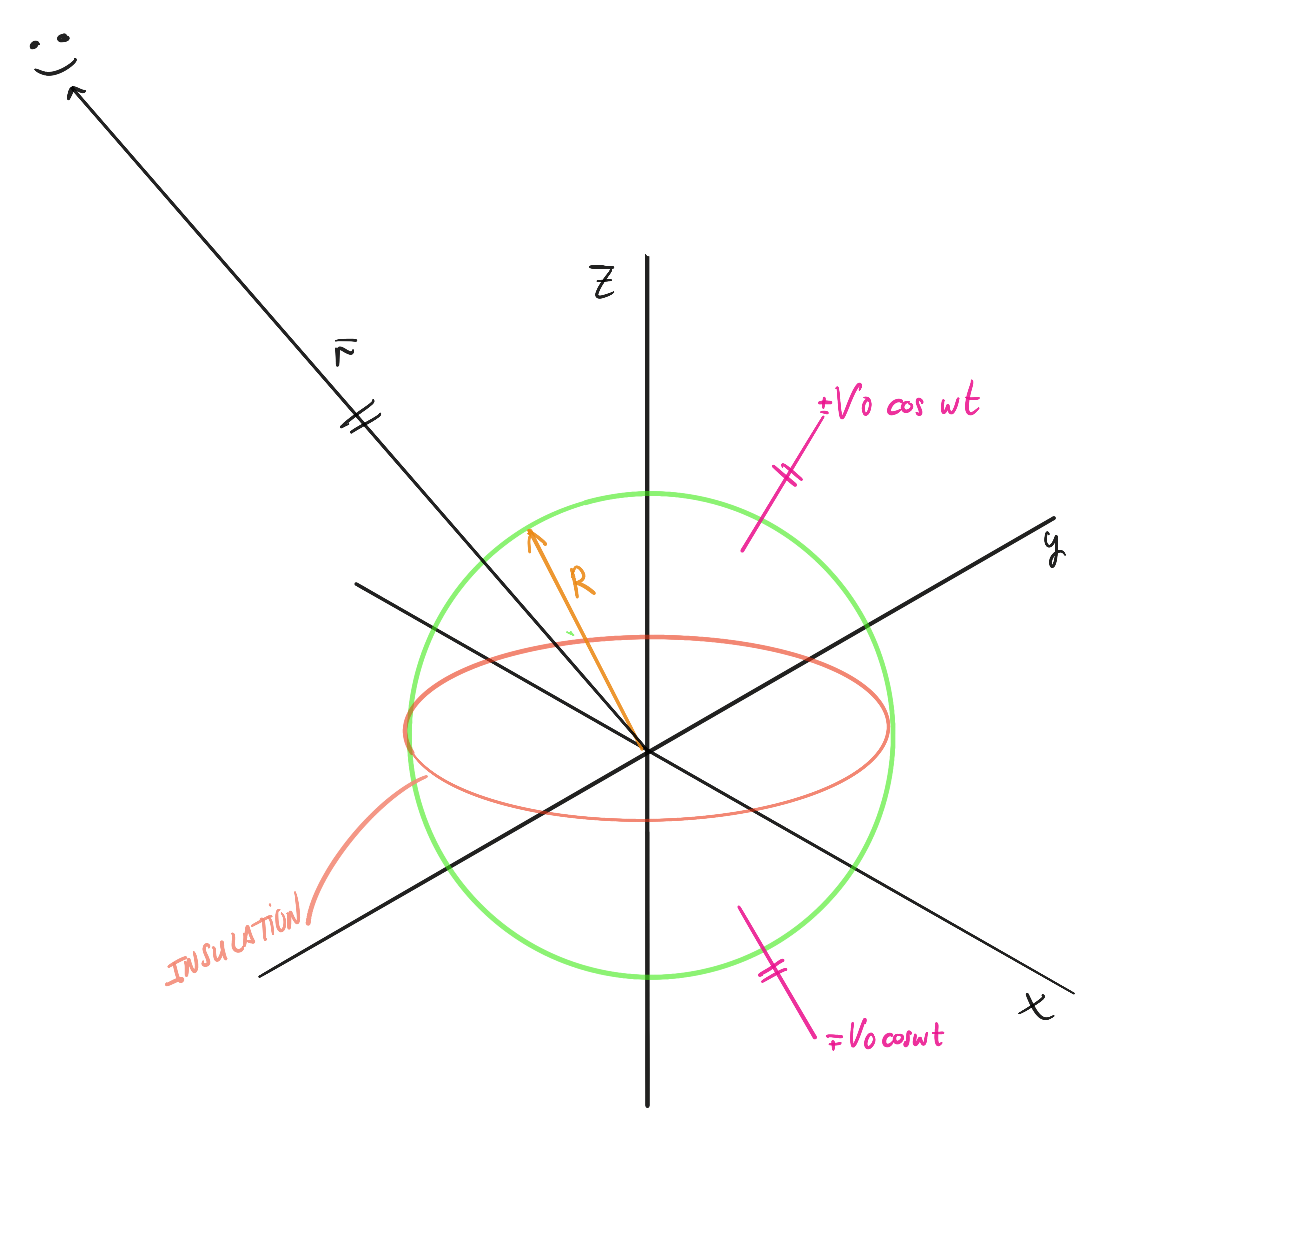
\includegraphics[width=8cm]{figures/Metallicshells.png}
	\centering
	\caption{The metallic shells with oscillating potentials.}
\end{figure}

One can derive the potential for this system using Green functions and proper boundary conditions. Also, one can find an explicit expression for this potential in Jackson (section 2.7, pg. 64), which is:

\begin{equation}
	\Phi (r, \theta, \phi) = \frac{3 V_{\pm} R^{2}}{2 r^{2}} \left(\frac{r^{3}(r^{2}-R^{2})}{(r^{2} + R^{2})^{\tfrac{5}{2}}}\right)\cos\theta \cdots
\end{equation}

Where $\cdots$ mean that there are higher order corrections. Recall that $r$ is the observation position, $R$ stands for the radius of the shells and $V_{\pm}$ is a short-hand notation for $V_{0}\cos \omega t$.

If we are in the long-wavelength limit ($r\gg \omega \gg R$), it also means that we have $r\gg R$, so we can simplify previous expression by:

\begin{equation}
	\begin{split}
		\Phi (r, \theta, \phi)|_{r\gg R} &= \frac{3 V_{\pm} R^{2}}{2 r^{2}} \left(\frac{r^{3}(r^{2}-\cancel{R^{2}})}{(r^{2} + \cancel{R^{2}})^{\tfrac{5}{2}}}\right)\cos\theta \cdots =\\
		&= \frac{\pm 3 V_{0} \cos \omega t \: R^{2}}{2 r^{2}}\cos \theta.
	\end{split}
\end{equation}

So we now have an appropriated approximation of the potential for this system. Then we can start computing the electric dipole.  At this stage, we can exploit the fact that the potential generated by a regular dipole is:

\begin{equation}\label{generalpotential}
	\Phi (r, \theta, \phi) = \frac{1}{4\pi \epsilon_{0}} \left(\sum_{i} \frac{q_{i}}{r} + \sum_{i} \frac{\vec{p}_{i}\cdot \vec{x}_{i}}{r^{3} } +\cdots \right).
\end{equation}

So, if we think in terms of being far, far away, we can think of the metallic shell system with oscillating potentials as dipole generated by two "charges" at the origin. But here we have no charges! (So the first term in (\ref{generalpotential}) is 0). If we compare (\ref{generalpotential}) with the simplified potential in the long wavelength limit, we find:

\begin{equation}
	\begin{split}
		\Phi (r, \theta, \phi) &= \frac{1}{4\pi \epsilon_{0}} \left( \frac{p \: r \: \cos \theta}{r^{3}}\right) = \frac{3 V_{\pm} R^{2}}{2 r^{2}} \cos \theta \rightarrow \\
		\vec{p} &= 6 \pi V_{\pm} R^{2} \hat{z}.
	\end{split}
\end{equation}

Where, keeping the analogy with the dipole generated by two charges at the origin, we can ensure a $\hat{z}$ orientation of this one. This will be the first step to obtain the radiation field and the radiated power.

$\mathbf{E,H}$ fields of a radiating system are given by:

\begin{equation}
	\begin{split}
		\mathbf{H} &= \frac{c k^{2}}{4\pi}(\vec{n}\times \vec{p})\frac{e^{ikr}}{r}\left(1 + \frac{1}{ikr}\right),\\
		\mathbf{E} &= \frac{1}{4\pi \epsilon_{0}}\left(k^{2}(\vec{n}\times \vec{p})\times \vec{n}\: \frac{e^{ikr}}{r} + \left[3\vec{n}(\vec{n}\cdot\vec{p})-\vec{p}\right]\left(\tfrac{1}{r^{3}}- \tfrac{ik}{r^{2}}\right) e^{ikr}\right).
	\end{split}
\end{equation}

But in the long wavelength limit, and far far away, these two expressions get simplified to ($\tfrac{1}{r^{n}}$ will barely contribute):

\begin{equation}
	\begin{split}
		\mathbf{H} &= \frac{c k^{2}}{4\pi}(\vec{n}\times \vec{p})\frac{e^{ikr}}{r} =\cdots= \tfrac{3 c k^{2}}{2 r} \epsilon_{0} V R^{2} e^{ikr} \sin\theta \hat{\phi}\\
		\mathbf{E} &= \frac{1}{c \epsilon_{0}} \mathbf{H} \times \vec{n} =\cdots= -\tfrac{3k^{2}}{2r} V R^{2} e^{ikr} \sin \theta \hat{\theta}.
	\end{split}
\end{equation}

So with these two fields we just have to plug them inside the radiated power per solid angle to get:

\begin{equation}
	\frac{dP}{d\Omega} = \tfrac{1}{2} \Re \left[r^{2} \vec{n}\cdot \mathbf{E} \times \mathbf{H}^{*}\right] =\cdots = \tfrac{9}{8} c\epsilon_{0}k^{4}V^{2} R^{4} \sin^{2} \theta.
\end{equation}

So we just have to integrate over the solid angle to get the total radiated power as:

\begin{equation}
	\begin{split}
		P= \int d\Omega \: P &=  \underbrace{\tfrac{9}{8} c\epsilon_{0}k^{4}V^{2} R^{4}}_{A} \int \sin^{2} \theta \sin\theta d\theta \: d\phi,\\
		&= \frac{3\pi}{2}c\epsilon_{0}k^{4}V^{2} R^{4}.
	\end{split}
\end{equation}



\subsubsection{Electrostatic Potential from a Dipole}\label{Electrostatic Potential from a Dipole}

\textbf{\textcolor{red}{UNDER CONSTRUCTION}}

\subsubsection{Radiation Interference}\label{Radiation Interference}

\textbf{1):}

We can infer, without knowing too much about radiation, that if we have two types of dipoles radiating simultaneously, some sort of interference will appear (may be constructive, destructive...). Since the two sources emit in phase,

\begin{equation}
	\begin{split}
		\frac{d P}{d \Omega} &\propto |\hat{\mathbf{r}} \times (\mathbf{\alpha}_{elec}+\mathbf{\alpha}_{mag})|^{2} =\\
		&= (\hat{\mathbf{r}}\times\alpha_{elec})^{2} + (\hat{\mathbf{r}}\times\alpha_{mag})^{2} + 2\underbrace{(\hat{\mathbf{r}}\times\alpha_{elec})(\hat{\mathbf{r}}\times\alpha_{mag})}_{\text{interference term}}
	\end{split}
\end{equation}

The interference term can be further simplified using basic vector identities and it results to be:

\begin{equation}
	(\hat{\mathbf{r}} \times \mathbf{p}) \cdot[\hat{\mathbf{r}} \times(\mathbf{m} \times \hat{\mathbf{r}})]=(\hat{\mathbf{r}} \times \mathbf{p}) \cdot[\mathbf{m}-\hat{\mathbf{r}}(\hat{\mathbf{r}} \cdot \mathbf{m})]=(\hat{\mathbf{r}} \times \mathbf{p}) \cdot \mathbf{m}=\hat{\mathbf{r}} \cdot(\mathbf{p} \times \mathbf{m}).
\end{equation}

Which is 0 $\iff$ $\mathbf{p} \parallel \mathbf{m}$.

\textbf{2):}

If we want to check that the time-averaged total power emitted has no interference contribution, we have to integrate over the solid angle $\Omega$.

\begin{equation}
	\begin{split}
		P=\int d \Omega \frac{d P}{d \Omega} &\propto \int_{0}^{2 \pi} d \phi \int_{0}^{\pi} d \theta \: \hat{\mathbf{r}} \cdot(\mathbf{p} \times \mathbf{m})\: \sin \theta  \\
		&\propto \hat{\mathbf{r}}\cdot(\mathbf{p} \times \mathbf{m}) \int_{-\pi/2}^{\pi/2} d\theta \sin \theta=0.
	\end{split}
\end{equation}

A zero as big as a cathedral.\footnote{Basic Spanish say when you want to specify that something is quite big/notorious.} No interference contribution over the whole spaubsce.



\subsubsection{Sinusoidal thin Antenna}\label{Sinusoidal thin Antenna}
As always, let's start with a sketch of the system:

\begin{figure}[h]
	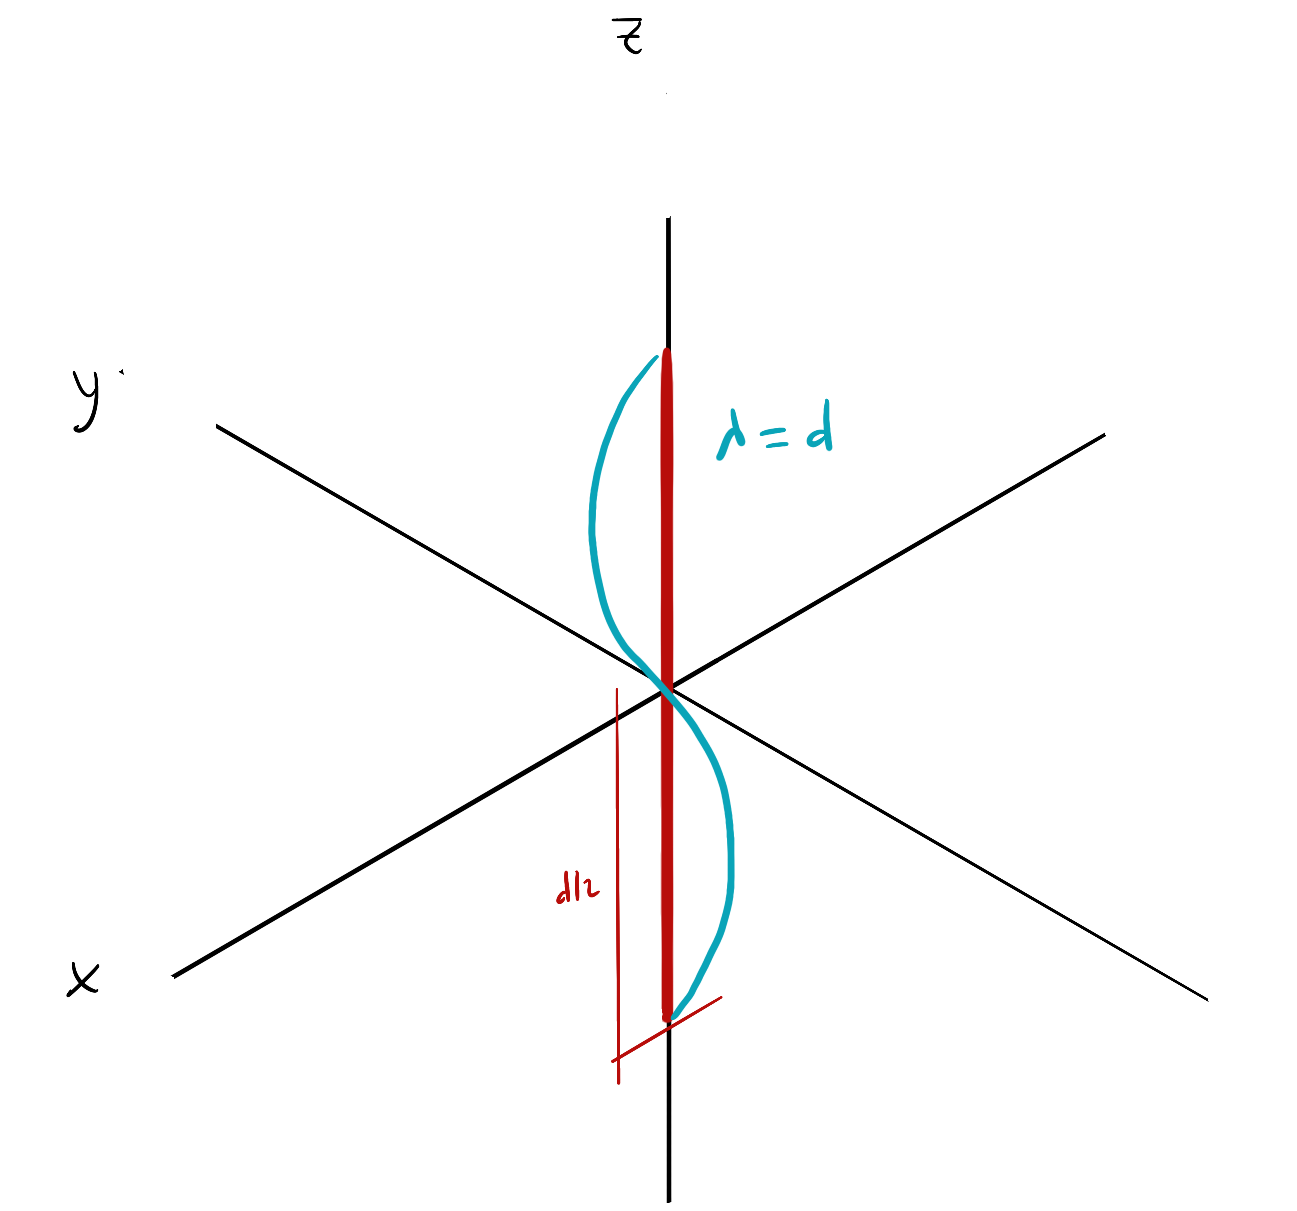
\includegraphics[width=8cm]{figures/sinuantenna.png}
	\centering
	\caption{Our simple antenna sample.}
\end{figure}

\textbf{a):}
	
Note that the current flows in opposite directions in the top and bottom half of this antenna (It is born at the centre and goes up and down). As a result, we may write the source current density using the Heaviside distribution as:

\begin{equation}
	\vec{J}(z)=\hat{z} I \sin (k z) \delta(x) \delta(y) \Theta(d / 2-|z|), \quad \quad \text{with}\quad  k=\frac{2 \pi}{d}.
\end{equation}

In the radiation zone, the vector potential is given by the well know expression:

\begin{equation}
	\begin{split}
		\vec{A}(\vec{x}) &=\frac{\mu_{0}}{4 \pi} \frac{e^{i k r}}{r} \int \vec{J}\left(\vec{x}^{\prime}\right) e^{-i k \hat{n} \cdot \vec{x}^{\prime}} d^{3} x^{\prime},\\
		&=\hat{z} \frac{\mu_{0} I}{4 \pi} \frac{e^{i k r}}{r} \int_{-d / 2}^{d / 2} \sin (k z) e^{-i k z \cos \theta} d z.
	\end{split}
\end{equation}

At this point, when integrating, we have to possible options:

\begin{itemize}
	\item To express the $\sin$ in terms of exponentials, rephrase, integrate and compose trigonometric functions again or...
	\item To perform a change of variables and use $\int_{-\pi}^{\pi}\sin(z) e^{-iaz}dz= \tfrac{2i \sin(\pi a)}{a^{2}-1} $.
\end{itemize}

All in all the result should be the same. Let's perform the first choice. Since the source current is odd under $z \rightarrow-z$, this integral may be written as:

\begin{equation}
	\begin{split}
		\vec{A} &=-\hat{z} \frac{i \mu_{0} I}{4 \pi} \frac{e^{i k r}}{r} \int_{0}^{d / 2} 2 \sin (k z) \sin (k z \cos \theta) d z =\\
		&=-\hat{z} \frac{i \mu_{0} I}{4 \pi} \frac{e^{i k r}}{r} \int_{0}^{d / 2}[\cos ((1-\cos \theta) k z)-\cos ((1+\cos \theta) k z)] d z= \\
		&=-\hat{z} \frac{i \mu_{0} I}{4 \pi} \frac{e^{i k r}}{k r}\left[\frac{1}{1-\cos \theta} \sin ((1-\cos \theta) k z)-\frac{1}{1+\cos \theta} \sin ((1+\cos \theta) k z)\right]_{0}^{d / 2}= \\
		&=-\hat{z} \frac{i \mu_{0} I}{2 \pi} \frac{e^{i k r}}{k r} \frac{\sin (\pi \cos \theta)}{\sin ^{2} \theta}.
	\end{split}
\end{equation}

To compute $H$ in the radiation zone, recall that $\vec{\nabla} \sim i k \hat{n}$, so:

\begin{equation}
	\vec{H}=\frac{i k}{\mu_{0}} \hat{n} \times \vec{A}=-\hat{\phi} \frac{I}{2 \pi} \frac{e^{i k r}}{r} \frac{\sin (\pi \cos \theta)}{\sin \theta}.
\end{equation}

where we used $\hat{n} \times \hat{z} \equiv \hat{r} \times \hat{z}=-\hat{\phi} \sin \theta$.  Then, the radiated power:

\begin{equation}
	\frac{d P}{d \Omega}= \frac{r^{2}}{2} \hat{n} \left(\vec{E} \times \vec{H}\right) = \underbrace{\frac{r^{2}}{2} \hat{n} \left(Z_{0}(\vec{H}\times \hat{n})\times\vec{H}\right)}_{\text{in the radiation zone.}} .
\end{equation}

Using some identities, this results into a radiated power of the form:

\begin{equation}
	\frac{d P}{d \Omega}=\frac{Z_{0} r^{2}}{2}|\vec{H}|^{2}=\frac{Z_{0}|I|^{2}}{8 \pi^{2}} \frac{\sin ^{2}(\pi \cos \theta)}{\sin ^{2} \theta}.
\end{equation}

\textbf{b):}

To compute the total radiated power we just have to integrate the previous result by the solid angle so:

\begin{equation}
	P = \int_{\Omega} \frac{dP}{d \Omega} d\Omega = \frac{Z_{0}I^{2}}{8}.
\end{equation}

\textbf{c):}

This part of the problem is more pure calculations. We need the definition of the dipoles and quadropoles, given by:

\begin{equation}
	\vec{p}=\int \vec{x} \: \rho\:  d^{3} x, \quad \quad \vec{m}=\frac{1}{2} \int \vec{x} \times \vec{J} d^{3} x, \quad \quad  
	Q_{i j}=\int\left(3 x_{i} x_{j}-r^{2} \delta_{i j}\right) \rho d^{3} x.
\end{equation}

To extract the charge density, we can use the equation of state $\vec{\nabla}\cdot J + \partial_{t} \rho =0$. Also, recall that $\vec{J}(t,\vec{x}) = \vec{J}(\vec{x}) e^{-i\omega t}$, so:

\begin{equation}
	\rho=\frac{1}{i \omega} \vec{\nabla} \cdot \vec{J}=\frac{1}{i \omega} \frac{d \vec{J}}{d z}=-\frac{i I}{c} \cos (k z) \delta(x) \delta(y) \Theta(d / 2-|z|)
\end{equation}

where we used $\omega=c k$. The electric dipole moment is then:

\begin{equation}
	\begin{split}
		\vec{p}=\int \vec{x} \rho d^{3} x&= \int dx \:dy \:dz \:(x \hat{x} + y \hat{y} + z \hat{z}) \:\frac{i I}{c} \cos (k z) \delta(x-0) \delta(y-0)=\\
		&=  -\hat{z} \frac{i I}{c} \int_{-d / 2}^{d / 2} z \cos (k z) d z=0
	\end{split}
\end{equation}

Of course, a simple symmetry argument under $z \rightarrow-z$ demonstrates that this electric dipole must vanish. The magnetic dipole moment also vanishes since:

\begin{equation}
	\vec{m}=\frac{1}{2} \int \vec{x} \times \vec{J} d^{3} x= \text{same story as before...}=\frac{I}{2} \int_{-d / 2}^{d / 2} \vec{z} \times[\hat{z} \sin (k z)] d z=0
\end{equation}

We are left with an electric quadrupole moment as:

\begin{equation}
	Q_{i j}=\int\left(3 x_{i} x_{j}-r^{2} \delta_{i j}\right) \rho d^{3} x.
\end{equation}

That gives us the expected $Q_{ij} = 0$ and:

\begin{equation}
	\begin{split}
		Q_{xx} = Q_{yy} = -\tfrac{1}{2} Q_{zz} &= -\frac{  I}{ic} \int_{-d / 2}^{d / 2} (3x_{i}^{2} - \sum x_{i}^{2})  \delta(x)\delta(y)\cos (k z) d z =\\
		&= \frac{- I d^{3}}{i c \pi^{2}}.
	\end{split}
\end{equation}




\subsubsection{Scattering in Solid Sphere}\label{Scattering in Solid Sphere}

We first have to understand what the set-up. Let's observe the following sketch.

\begin{figure}[h]
	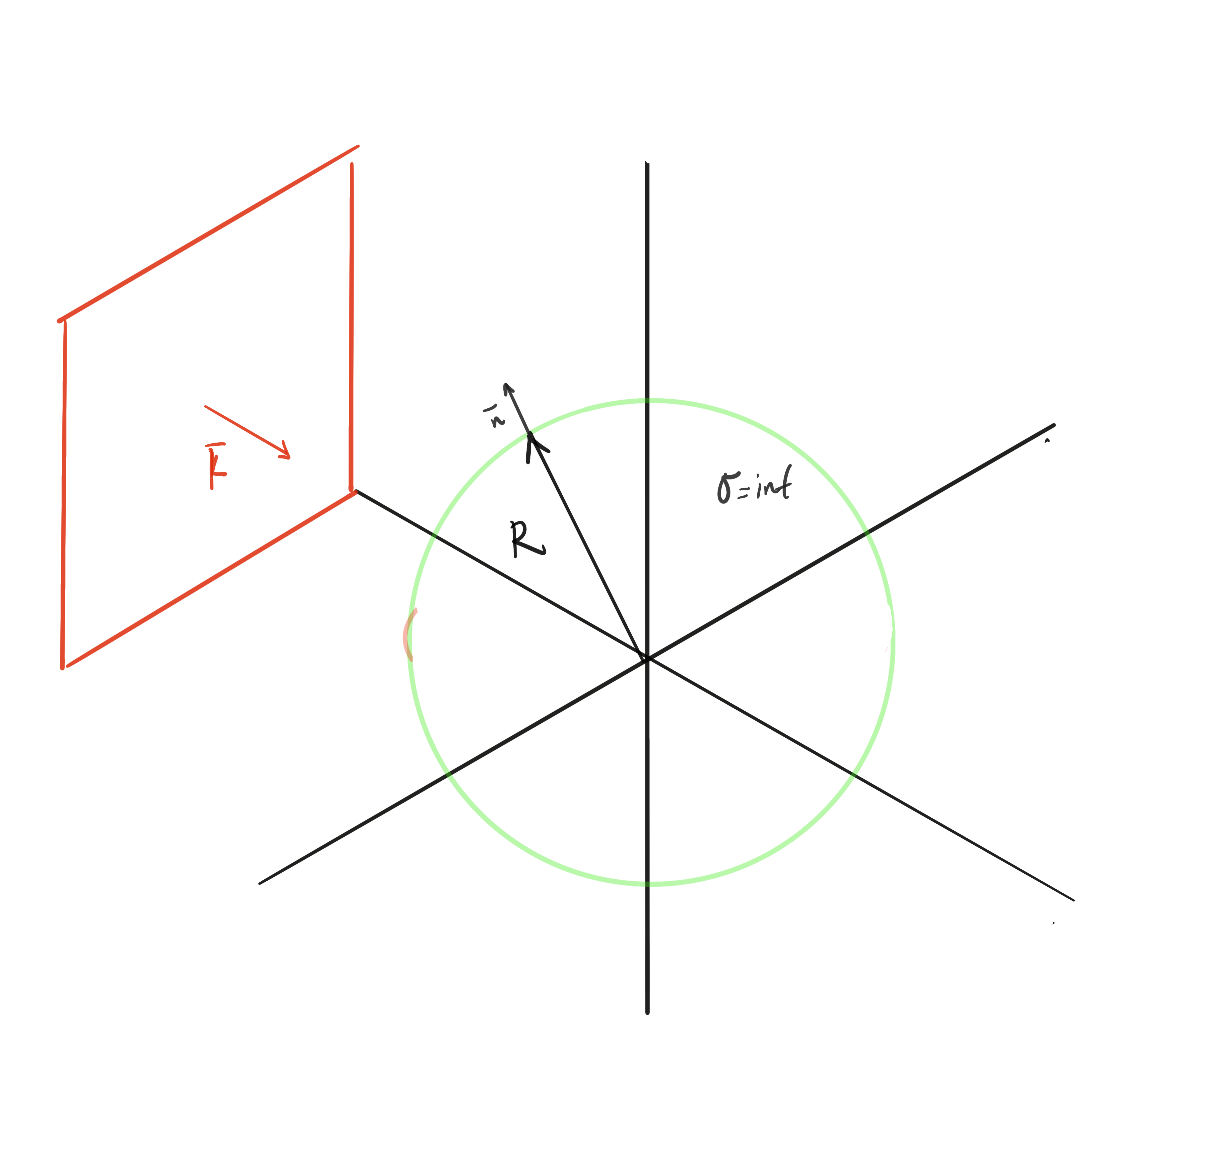
\includegraphics[width=8cm]{figures/Scatteringsphere.png}
	\centering
	\caption{A sphere being hit by a plane wave.}
\end{figure}

Then, let's proceed with the different parts of this problem.

\textbf{1):}

Assuming that conductivity $\sigma$ is infinite, we then just realise that there will be no fields inside the sphere, hence no current $J$ inside this one. In the same spirit as in the electric case, one can think in terms of a "magnetic" potential $\phi_{M}$, whose divergence will generate the magnetic field $\mathbf{B}$ around the sphere surface. In order to find this potential, let's use the multipole expansion of it and some boundary conditions. We know that the most general potential expansion looks like:
	
\begin{equation}
	\Phi(\mathbf{r},\theta, \phi)=\sum_{\ell=0}^{\infty}\left( A_{\ell } r^{\ell}  + \frac{B_{\ell }}{r^{\ell+1}} \right) P_{\ell}(\cos\theta).
\end{equation}

And what are the boundary conditions we know? That the potential on the surface should be 0 and $-B_{0}\:z$\footnote{the field carried from the plane wave, but reflected.} when $r\gg R$. Then, the second boundary condition help us fix the first linear coefficient as:

\begin{equation}
	\begin{split}
		\phi_{M}|_{r\gg R} = -B_{0} r\: \cos\theta &= \sum_{\ell=0}^{\infty}\left( A_{\ell } r^{\ell}  + \underbrace{\frac{B_{\ell }}{r^{\ell+1}}}_{r\gg R} \right) P_{\ell}(\cos\theta) =,\\
		-B_{0} r\: \cos\theta &= \sum_{\ell=0}^{\infty}\left( A_{\ell } r^{\ell} \right) P_{\ell}(\cos\theta) = A_{1}\: r^{1} \cos\theta=,\\
		B_{0} &= A_{1}.
	\end{split}	 
\end{equation}

There is a missing boundary condition that used now can shed some light on the sub-leading coefficient of this expansion. Recall that for a perfect conducting spherical surface one has $B_{\perp} =0$ when $r=R$. And recall that $-\vec{\nabla} \phi_{M} = \mathbf{B}$, so:

\begin{equation}
	\begin{split}
		0= -\partial_{r}|_{r=R} &= 	-\partial_{r}\left(-B_{0}\: r\cos\theta + \sum_{\ell=0}^{\infty}\frac{ B_{\ell}}{ r^{\ell + 1}} P_{\ell}(\cos\theta)\right)=\\
		-B_{0} \cos\theta &= \sum_{\ell=0}^{\infty}\frac{(\ell+1) R^{\ell}B_{\ell }}{ R^{2 \ell + 2}} P_{\ell}(\cos\theta)=\\
		B_{1} &= -\frac{R^{3} B_{0}}{2}.
	\end{split}
\end{equation}

So the first leading order of the "magnetic" potential are:

\begin{equation}
	\begin{split}
		\phi_{M}(r,\theta) &= -B_{0}\: r \cos\theta \left(1+ \tfrac{R^{3}}{2r^{3}}\right) \rightarrow \\
		\phi_{M}(z) &= -B_{0}\: z\left(1+ \tfrac{R^{3}}{2r^{3}}\right).
	\end{split}
\end{equation}

Which will result into the following magnetic field:

\begin{equation}
	\mathbf{B}= -\vec{\nabla}\phi_{M} = B_{0}\left(1- \tfrac{R^{3}}{2}\left(\tfrac{3\hat{r}\:z^{2}-1}{r^{3}}\right)\right).
\end{equation}

\textbf{2):}

The absorption cross section is the ratio between the power loss and the intensity of the plane wave.  Let's compute the power loss by:

\begin{equation}
	\begin{split}
		\frac{P_{\mathrm{loss}}}{\underbrace{d a}}_{\text{area}} &= \frac{1}{2 \sigma \delta}  \left|\hat{n} \times \tfrac{\mathbf{B}}{\mu}\right|^{2} = \\
		&= \frac{1}{2\sigma\delta} \left| \hat{r} \times B_{0}\left(1- \tfrac{R^{3}}{2}\left(\tfrac{3\hat{r}\:z^{2}-1}{r^{3}}\right)\right)\right|^{2}=\\
		&= \frac{B_{0}^{2}}{2\mu^{2}}\left( 1+ \tfrac{R^{3}}{2r^{3}} \right)^{2} \sin^{2}\theta \:\hat{\phi}.
	\end{split}
\end{equation}

So integrating this power loss over the whole area of the sphere we get:

\begin{equation}
	\begin{split}
		P &= \int_{\text{Area}} \: \frac{B_{0}^{2}}{2\mu^{2}}\left( 1+ \tfrac{R^{3}}{2r^{3}} \right)^{2} \sin^{2}\theta R^{2} \sin\theta d\theta d\phi=\\
		&\\
		&= \frac{3B_{0}^{2}R^{2}\pi}{\sigma \delta \mu^{2}}.
	\end{split}
\end{equation}

We only need to know the intensity of the incident plane wave. One can obtain this from the strength of both fields carried by the wave, which is given by the energy average of a wave, as:

\begin{equation}
	\left\langle S \right\rangle = I = \tfrac{\epsilon_{0}}{2}\left|\mathbf{E}\right|^{2} = \tfrac{1}{2\mu_{0}} \left|B_{0}\right|^{2}
\end{equation}

Then, the cross section is finally given by:

\begin{equation}\label{cross}
	\sigma_{\text{cross}} = \frac{P_{\mathrm{loss}}}{I} = \frac{6R^{2}\pi}{\sigma \delta \mu}.
\end{equation}

Observe that expression (\ref{cross}) does not depend on the fields that the wave carries, but the properties of the object is scattered on. In this case, the radius, the conductivity and the skin depth..ubs.

\subsubsection{Aperture (Science)}\label{Aperture (Science)}
\textbf{\textcolor{red}{UNDER CONSTRUCTION}}


\subsubsection{Born Scattering from a Dielectric Cube}\label{Born Scattering from a Dielectric Cube}

\textbf{1):}

The first thing we have to notice in order to be able to approximate "a la Born" is that $\mathbf{E}$ inside a dielectric material has to be very similar to the incident electric field $\mathbf{E}$. If this then the case, we know that $\mathbf{J} \propto \mathbf{E}$. In order to simplify the fore coming expression, let us write $\mathbf{q}=\mathbf{k}-\mathbf{k}_{0}$ as the difference between the incoming and outgoing scattering wave vectors $\left(\omega=c k=c k_{0}\right)$. Then, the approximated cross section is given by:

\begin{equation}
	\frac{d \sigma_{\text {Born }}}{d \Omega}=\left(\frac{k_{0}^{2}\: V\: \chi_{e}}{4 \pi}\right)^{2}\left|\hat{\mathbf{k}} \times \hat{\mathbf{E}}_{0}\right|^{2}\left|\int_{V} d^{3} r^{\prime} \exp \left(i \mathbf{q} \cdot \mathbf{r}^{\prime}\right)\right|^{2}.
\end{equation}

Where $\chi$ is the susceptibility of the material of the cube. The pesky integral we have to compute goes as:

\begin{equation}
	\int_{V} d^{3} r^{\prime} \exp \left(i \mathbf{q} \cdot \mathbf{r}^{\prime}\right)=\int_{0}^{a} d x^{\prime} \exp \left(i q_{x} x^{\prime}\right) \times \int_{0}^{a} d y^{\prime} \exp \left(i q_{y} y^{\prime}\right) \times \int_{0}^{a} d z^{\prime} \exp \left(i q_{z} z^{\prime}\right).
\end{equation}

But we have to realise the following technical computation.
	
\begin{equation}
	\begin{split}
		\int_{0}^{a} d x^{\prime} \exp \left(i q_{x} x^{\prime}\right)&= \frac{e^{i q_{x} x}}{i q_{x}} |^{a}_{0}=\\
		&= \underbrace{\tfrac{e^{iq_{x}a}}{i q_{x}} - 1}_{\text{extract $1/2$ of the exp}} = \tfrac{e^{iq_{x}a/2}}{i q_{x}}(\underbrace{e^{i q_{x}a/2}-e^{-i q_{x}a/2}}_{=\sin \cdots})=\\
		&=2 e^{ \left(-i q_{x} a / 2\right)} \frac{\sin \left(q_{x} a / 2\right)}{q_{x} a / 2}
	\end{split}
\end{equation}

Which works exactly the same for $y,z$ components. Then, the cross section looks like:

\begin{equation}
	\frac{d \sigma_{\text {Born }}}{d \Omega}=\left(\frac{k_{0}^{2} V \chi_{e}}{4 \pi}\right)^{2}\left|\hat{\mathbf{k}} \times \hat{\mathbf{E}}_{0}\right|^{2}\left[8\: \frac{\sin \left(q_{x} a / 2\right)}{q_{x} a / 2} \frac{\sin \left(q_{y} a / 2\right)}{q_{y} a / 2} \frac{\sin \left(q_{z} a / 2\right)}{q_{z} a / 2}\right]^{2}
\end{equation}

\textbf{2):}

Now we have to show that $\sigma \approx \tfrac{1}{4}k^{2}a^{4}\chi^{2}$ when $ka\gg 1$. Let $\mathrm{k}_{0}=\hat{\mathrm{z}}$ and $\mathrm{E}_{0}=\hat{\mathrm{x}}$. When $k a \gg 1$, near-forward scattering dominates and $\left|\hat{\mathbf{k}} \times \hat{\mathbf{E}}_{0}\right| \approx\left|\hat{\mathbf{k}}_{0} \times \hat{\mathbf{E}}_{0}\right|=1$. The sketch below shows that, in the same limit, the area element $k^{2}\Omega_{\mathrm{k}}$ is essentially the area $d q_{x} d q_{y}$ of a circular disk perpendicular\footnote{Basically, try to imagine the to-be-scattered wave as a spherical one and the surface of this that will interact with the cube is given such that there is not too much difference of $k$ in $z$ direction.} to $\mathrm{k}_{0}$:

\begin{equation}
	d S_{\mathrm{k}}=k^{2} d \Omega_{\mathrm{k}} \approx d q_{x} d q_{y}.
\end{equation}

\begin{figure}[h]
	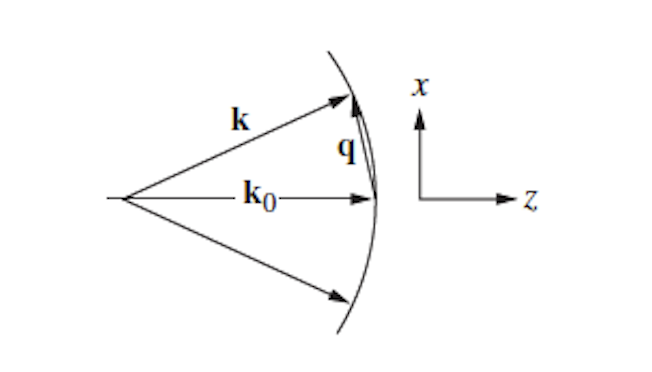
\includegraphics[width=8cm]{figures/cubegeometry.png}
	\centering
	\caption{The important $k$ to give an accurate approximation.}
\end{figure}

Therefore, in the $k a \gg 1$ limit when $q_{z} \rightarrow 0$, the fact that $k_{0}=k$ means that:

\begin{equation}
	\lim _{k a \gg 1} \sigma_{\text {Born }}=\lim _{k a \gg 1} \int d \Omega_{\mathrm{k}} \frac{d \sigma_{\text {Born }}}{d \Omega_{\mathrm{k}}} \approx \lim _{k a \gg 1}\left(\frac{k V \chi_{e}}{4 \pi}\right)^{2} \int d q_{x} \frac{\sin ^{2}\left(q_{x} a / 2\right)}{\left(q_{x} a / 2\right)^{2}} \int d q_{y} \frac{\sin ^{2}\left(q_{y} a / 2\right)}{\left(q_{y} a / 2\right)^{2}}.
\end{equation}

Here we have to be careful. The integrals are mainly dominated by contributions when $q_{x}, q_{y} \sim 1 / a$ so the limits can be extended to $\pm \infty$\footnote{The peak of contribution happens at $1/a$ for the momenta with the remaing values of $q_{i}$ barely contributing to the situation. Expanding the integration to all $\mathrm{R}$ we simplify our life.}with little loss of accuracy. Therefore,

\begin{equation}
	\lim _{k a \gg 1} \sigma_{\text {Born }}=\frac{k^{2} a^{4} \chi_{e}^{2}}{4 \pi^{2}}\left[\int_{-\infty}^{\infty} \frac{\sin ^{2} u}{u^{2}}\right]^{2}\approx\frac{k^{2} a^{4} \chi_{e}^{2}}{4}.
\end{equation}

\textbf{3):}

From the definition of the cross section and the result of part (1),

\begin{equation}
	\frac{E_{\mathrm{rad}}}{E_{0}} \approx \frac{1}{r} \sqrt{\frac{d \sigma}{d \Omega}} \approx \frac{k^{2} a^{3} \chi_{e}}{4 \pi r}\left|\frac{\sin \left(q_{x} a / 2\right)}{q_{x} a / 2} \frac{\sin \left(q_{y} a / 2\right)}{q_{y} a / 2} \frac{\sin \left(q_{z} a / 2\right)}{q_{z} a / 2}\right|.
\end{equation}

The absolute-value term gets no larger than one. Therefore, with $r=a$, the weak scattering criterion is indeed

\begin{equation}
	1 \gg k^{2} a^{2} \chi_{e}=\sigma_{\mathrm{Born}} / a^{2} \chi_{e}.
\end{equation}

\subsubsection{E: Two Antennas Sitting Together}\label{E: Two Antennas Sitting Together}

\textbf{1):}

As almost all radiation problems, let's start computing the different dipole momenta for each of the components of the system. Recall that when integrating we only care about the spatial components. The magnetic dipole for the loop antenna is:

\begin{equation}
	\vec{m}_{\mathrm{loop}} = \tfrac{1}{2} \int \vec{x}\times \vec{J}(\vec{x}) d^{3} x = I \times \text{Area}_{S_{2}} \cdot \hat{n} = I_{0} \pi a^{2} \hat{z}.
\end{equation}

Where we shall recall that for a close loop we can use the previous magnetic dipole simplification. Also, the dipole will be pointing perpendicular to the surface of the area. For the electric dipole of the straight antenna we find:

\begin{equation}
	\vec{P}_{\mathrm{ant}} = \int \vec{x}\cdot \rho (\vec{x})d^{3}x = \int^{0}_{-a}  -i\lambda_{0}\: z \: dz + \int^{a}_{0} i\lambda_{0} \:  z \: dz = i\lambda_{0}\: a^{2} \hat{z}.
\end{equation}

\textbf{2):}

Assuming that the emitted wavelength is greater than the size of the system and that we are far far away of the source, we can just drop terms with a $\tfrac{1}{r^{n}}$ dependence in the vector potential expression $\mathbf{A}$. Also, as we have two antennas, whose dipoles are aligned along the $z$-axis, the total vector potential will be no more than a linear combination of each of the parts as:

\begin{equation}
	\begin{split}
		\mathbf{A}_{total} &= \mathbf{A}_{ant}(\vec{x}) + \mathbf{A}_{loop}(\vec{x}) =\\
		&= \frac{ik\mu_{0}}{4\pi}(\hat{r}\times\vec{m})\frac{e^{ikr}}{r} - \frac{i\mu_{0}\omega}{4\pi}\vec{p} \frac{e^{ikr}}{r}=\\
		&= \frac{i\mu_{0}\omega e^{ikr}}{4\pi \:r} \left(\tfrac{1}{c}\pi I_{0} a^{2} \hat{r}\times \vec{z} - i\lambda_{0}a^{2}\hat{z}\right).
	\end{split}
\end{equation}

We will leave this expression for future convenience in the computation.

\textbf{3):}
	
Same principle as before, $\mathbf{E}$ and $\mathbf{B}$ will have contributions from both antennas. In this case, let's start with:

\begin{equation}\label{magneticfield}
	\begin{split}
		\mathbf{H}_{tot} &= \mathbf{H}_{ant} + \mathbf{H}_{loop}=\\
		&= \frac{e^{ikr}k^{2}}{4\pi r} \left(c(\hat{r}\times \vec{p}) - (\hat{r}\times \vec{m})\times \hat{r}\right) = \text{use vector identities} = \\
		&= \frac{e^{ikr}k^{2}}{4\pi r}\left(c(\hat{r}\times \hat{z})\: i\lambda_{0}a^{2} - \pi I_{0} a^{2}\hat{z}- \pi I_{0}a^{2}\underbrace{\cos\theta \: \hat{r}}_{\vec{m}\cdot \hat{r}= \cos\theta}\right).
	\end{split}
\end{equation}

Then it is easy to consider that $\mathbf{B} = \mu_{0} \mathbf{H}_{tot}$. For the electric field, as we are in the radiation zone, we know that:

\begin{equation}
	\begin{split}
		\mathbf{E}_{tot} &= Z_{0} \mathbf{H}_{tot} \times \hat{r} = \\
		&= \sqrt{\tfrac{\mu_{0}}{\epsilon_{0}}}k^{2} \frac{e^{ikr}}{4\pi r}\left(c\: i\lambda_{0}a^{2}(\hat{r}\times\vec{z})\times\hat{r} + \pi I_{0}a^{2}\hat{r}\times \hat{z}- \cancel{\hat{r}\times\hat{r}}\right)=\\
		&\\
		&=\text{Again, use some vector identities to simplify...}=\\
		&\\
		&=\frac{-k^{2}}{4\pi r}\sqrt{\tfrac{\mu_{0}}{\epsilon_{0}}}\frac{e^{ikr}}{r}(i\: c\lambda_{0}a^{2}(\hat{z}-\hat{r})).
	\end{split}
\end{equation}

Then, finally, we are prepared to compute the power emitted per unit of solid angle...

\textbf{4):}

So we know it expression as:

\begin{equation}
	\begin{split}
		\left\langle \frac{dP}{d\Omega}\right\rangle &= \frac{1}{2}\Re\left[r^{2} \hat{r}\cdot(\vec{E}\times \vec{H}^{*})\right] =\\
		&= \frac{1}{2}\Re\left[r^{2} \hat{r}\cdot\left(\sqrt{\tfrac{\mu_{0}}{\epsilon_{0}}}\left(\vec{H}\times \hat{r}\right)\times \vec{H}^{*}\right)\right]=\\
		&\\
		&= \text{use vector identities}=\\
		&\\
		&= \frac{1}{2}\Re\left[r^{2} \sqrt{\tfrac{\mu_{0}}{\epsilon_{0}}} \vec{H}\cdot \vec{H}^{*})\right].
	\end{split}
\end{equation}

We can suspect what is about to come. One has to compute the conjugated square of expression (\ref{magneticfield}). Grab a coffee, keep calm and compute with ease and patience. A result of the following form should pop up as:

\begin{equation}
	\left\langle \frac{dP}{d\Omega}\right\rangle = \sqrt{\tfrac{\mu_{0}}{\epsilon_{0}}} \frac{k^{4}}{16\pi^{2}} \left(c^{2}\lambda_{0}^{2}a^{4} \underbrace{(\vec{r}\times \hat{z})^{2}}_{1-(\vec{r}\cdot\hat{z})^{2}} + 2 \pi^{2} I_{0}^{2}a^{4}(1 + \underbrace{\hat{z}\cdot \vec{r}}_{-\cos\theta})\right).
\end{equation}

We are asked to give the answer as a function of the angle $\theta$. In order to simplify further the previous expression, recall that $\cos\theta = 1- 2\sin^{2}\theta/2$. With this in mind, the final result looks like:

\begin{equation}
	\left\langle \frac{dP}{d\Omega}\right\rangle =	\sqrt{\tfrac{\mu_{0}}{\epsilon_{0}}} \frac{k^{4}a^{4}}{32\pi^{2}} \left(c^{2}\lambda_{0}^{2} \sin^{2}\theta + 4 \pi^{2} I_{0}^{2}\sin^{2}\tfrac{\theta}{2}\right).
\end{equation}


\subsubsection{E: One... Err, Two Antennas}\label{E: Onubse... Err, Two Antennas}
\textbf{\textcolor{red}{UNDER CONSTRUCTION}}

\subsubsection{E : Who bent my Antenna?}\label{E : Who bent my Antenna?}

\textbf{1):}

This first part of the problem is just a warm up for what is about to come. Let's start computing the magnetic dipole. Careful here; We cannot assume a whole curved antenna, as there is a gap at $\pi$, that we shall not integrate over.  It is useful to move to cylindrical coordinates when computing in this exercise. Then we have:

\begin{equation}
	\begin{split}
		\vec{m} &= \tfrac{1}{2}\int d^{3}x \:\vec{x} \times \vec{J} = \tfrac{1}{2}\int d^{3}x \:( r, \alpha, 0) \times (0, I,0 ) =\\
		&= I_{0} a^{2} \hat{x} \int_{\pi}^{-\pi} d\alpha (\pi - |\alpha|) = \pi^{2} I_{0} a^{2} \hat{x}. 
	\end{split}
\end{equation}

To find the electric dipole we need first to know the charge density. This one can be extracted from the continuity equation as:

\begin{equation}
	\vec{\nabla}\cdot \vec{J} + \partial_{t} \rho =0 \rightarrow \lambda = \tfrac{-i}{a \omega} \partial_{\alpha} (I_{0}(\pi - |\alpha|))
\end{equation}

Which depends on the value of $\alpha$ (Recall that it is fed with a RF signal at $\alpha =0$). This means:

\begin{equation}
	\lambda  = \left\{\begin{array}{ll}
		\frac{i}{a \omega} I_{0} & 0 < \alpha < \pi, \\
		\frac{-i}{a \omega} I_{0} & -\pi<x <0.
	\end{array}\right.
\end{equation}

By symmetry $\vec{p}$ is in the $\hat{z}$ direction as:

\begin{equation}
	\vec{p} = \int d^{3}x \: \lambda \: \hat{z} = \tfrac{2i}{\omega} I_{0} a \hat{z} \: \int_{0}^{\pi} d\alpha \sin \alpha = \tfrac{4i}{\omega} I_{0} a \hat{z}.
\end{equation}

\textbf{2):}
	
At this point we could compute each of the contributions for each dipole to the vector field... Or we can be intelligent and save some time and brain cells by doing the following. We know that the vector potential is:

\begin{equation}
	\begin{split}
		\mathbf{A}(\vec{x})_{p} &= - \frac{i\mu_{0}\overbrace{\omega}^{c= k \omega}}{4\pi} \: \vec{p} \frac{e^{ikr}}{r},\\
		\mathbf{A}(\vec{x})_{m} &=  \frac{ik\mu_{0}}{4\pi} \vec{r}\times \vec{m}\left(1- \frac{1}{ikr}\right) \frac{e^{ikr}}{r}.\\
	\end{split}
\end{equation}

So the sum of both of them in the radiation zone (a.k.a big $r$ so drop terms $\propto \tfrac{1}{r}$) will yield the following result:

\begin{equation}
	\mathbf{A}(\vec{x}) =  \frac{ik\mu_{0}}{4\pi}\left( \vec{r}\times \vec{m} - c\vec{p}\right)\frac{e^{ikr}}{r} = \frac{i\mu_{0}}{4\pi} \: I_{0}k a \left(\pi^{2} k a(\hat{r}\times \hat{x}) - 4i \hat{z}\right)\frac{e^{ikr}}{r}.
\end{equation}

Observe that we have left the vector products as a formal expression. This has been done so we can exploit its identities later. With this expression in our power, is time to compute the fields.

\textbf{3):}

The fields are given by:

\begin{equation}
	\begin{split}
		\mathbf{B} &= \vec{\nabla}\times \vec{A} =,\\
		&=\frac{\mu_{0}}{4\pi} \: I_{0}k a \left(\pi^{2} k a\hat{r}\times(\hat{r}\times \hat{x}) + 4i\hat{r}\times \hat{z}\right)\frac{e^{ikr}}{r}.
	\end{split}
\end{equation}

And the Electric field is (in the radiation zone):

\begin{equation}
	\begin{split}
		\mathbf{E} &= c^{2} \tfrac{i}{\omega} \vec{\nabla} \times \vec{B} =,\\
		&=\frac{c\mu_{0}}{4\pi} \: I_{0}k a \left(\pi^{2} k a(\hat{x}\times \hat{r}) + 4i\hat{r}\times(\hat{z}\times \hat{r})\right)\frac{e^{ikr}}{r}.
	\end{split}
\end{equation}

\textbf{4):}

Finally, we have all the tools to compute the power emitted by solid angle. Recall that this is given by:

\begin{equation}\label{radiated}
	\frac{dP}{d\Omega} = \frac{r^{2}}{2\mu_{0}} \hat{r}\cdot \Re \left[\mathbf{E} \times \mathbf{B}^{*}\right] = \text{radiation zone} = \frac{r^{2}}{2\mu_{0}c} \left(\vec{E}\cdot\vec{E}^{*}\right).
\end{equation}

This forces us to carefully compute the set of vector products in the electric field. With some calm (and vector identities) we can find that:

\begin{equation}
	\begin{split}
		|\left(\pi^{2} k a(\hat{x}\times \hat{r}) + 4i\hat{r}\times(\hat{z}\times \hat{r})\right)|^{2} &=  \pi^{4} k^{2} a^{2}(\hat{x}\times \hat{r})(\hat{x}\times \hat{r}) + 16(\hat{z} - \hat{r}(\hat{r}\cdot \hat{z}))^{2} =\\
		&= \pi^{4} k^{2} a^{2}(1- (\hat{x}\cdot \hat{r})^{2}) + 16(1 - (\hat{r}\cdot \hat{z})^{2}) =,\\
		&= \pi^{4} k^{2} a^{2}(1- (\sin \theta \cos \phi)^{2}) + 16(1 - (\cos \theta)^{2}).
	\end{split}
\end{equation}

Plugging this back into expression (\ref{radiated}) we find:

\begin{equation}
	\frac{dP}{d\Omega} =  \frac{c\mu_{0}}{32 \pi^{2}} (I_{0} k a)^{2}\left(\pi^{4} k^{2} a^{2}(1- (\sin \theta \cos \phi)^{2}) + 16\sin\theta^{2})\right).
\end{equation}

